\chapter{Upiti nad stablom}

\index{upit nad stablom}

U ovom poglavlju razmatramo tehnike za
obradu upita nad
podstablima i putovima korijenskog stabla.
Primjeri takvih upita su:

\begin{itemize}
\item koji je $k$-ti predak čvora?
\item kolika je suma vrijednosti u podstablu čvora?
\item kolika je suma vrijednosti na putu između dvaju čvorova?
\item koji je najniži zajednički predak dvaju čvorova?
\end{itemize}

\section{Pronalaženje predaka}

\index{predak}

$k$-ti \key{predak} čvora $x$ u korijenskom stablu
je čvor do kojeg dolazimo ako se pomaknemo $k$
razina prema gore od $x$.
Neka $\texttt{ancestor}(x,k)$ označava $k$-tog pretka čvora $x$
(ili $0$ ako takav predak ne postoji).
Na primjer, u sljedećem stablu vrijedi
$\texttt{ancestor}(2,1)=1$ i $\texttt{ancestor}(8,2)=4$.
\begin{center}
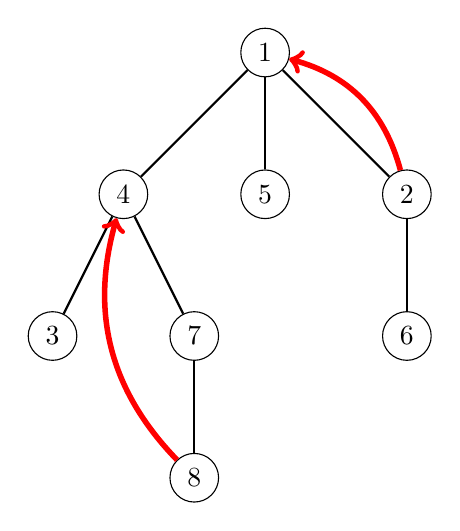
\begin{tikzpicture}[scale=0.9]
\node[draw, circle] (1) at (0,3) {$1$};
\node[draw, circle] (2) at (2,1) {$2$};
\node[draw, circle] (3) at (-2,1) {$4$};
\node[draw, circle] (4) at (0,1) {$5$};
\node[draw, circle] (5) at (2,-1) {$6$};
\node[draw, circle] (6) at (-3,-1) {$3$};
\node[draw, circle] (7) at (-1,-1) {$7$};
\node[draw, circle] (8) at (-1,-3) {$8$};
\path[draw,thick,-] (1) -- (2);
\path[draw,thick,-] (1) -- (3);
\path[draw,thick,-] (1) -- (4);
\path[draw,thick,-] (2) -- (5);
\path[draw,thick,-] (3) -- (6);
\path[draw,thick,-] (3) -- (7);
\path[draw,thick,-] (7) -- (8);

\path[draw=red,thick,->,line width=2pt] (8) edge [bend left] (3);
\path[draw=red,thick,->,line width=2pt] (2) edge [bend right] (1);
\end{tikzpicture}
\end{center}

Jednostavan način računanja bilo koje vrijednosti $\texttt{ancestor}(x,k)$
jest izvesti niz od $k$ pomaka u stablu.
Međutim, vremenska složenost te metode
je $O(k)$, što može biti sporo jer stablo s $n$
čvorova može sadržavati lanac od $n$ čvorova.

Srećom, koristeći tehniku sličnu onoj
iz poglavlja 16.3, bilo koja vrijednost $\texttt{ancestor}(x,k)$
može se efikasno izračunati u $O(\log k)$ vremenu
nakon predobrade.
Ideja je unaprijed izračunati sve vrijednosti $\texttt{ancestor}(x,k)$
gdje je $k \le n$ potencija broja dva.
Za gornje stablo te su vrijednosti
sljedeće:

\begin{center}
\begin{tabular}{r|rrrrrrrrr}
$x$ & 1 & 2 & 3 & 4 & 5 & 6 & 7 & 8 \\
\hline
$\texttt{ancestor}(x,1)$ & 0 & 1 & 4 & 1 & 1 & 2 & 4 & 7 \\
$\texttt{ancestor}(x,2)$ & 0 & 0 & 1 & 0 & 0 & 1 & 1 & 4 \\
$\texttt{ancestor}(x,4)$ & 0 & 0 & 0 & 0 & 0 & 0 & 0 & 0 \\
$\cdots$ \\
\end{tabular}
\end{center}

Predobrada traje $O(n \log n)$ vremena
jer se za svaki čvor računa $O(\log n)$ vrijednosti.
Nakon toga bilo koju vrijednost $\texttt{ancestor}(x,k)$ možemo izračunati
u $O(\log k)$ vremenu tako da $k$ prikažemo
kao sumu u kojoj je svaki pribrojnik potencija broja dva.

\section{Podstabla i putovi}

\index{niz obilaska stabla}

\key{Niz obilaska stabla} sadrži čvorove korijenskog stabla
onim redoslijedom kojim ih posjećuje pretraživanje u dubinu
koje kreće iz korijena.
Na primjer, u stablu
\begin{center}
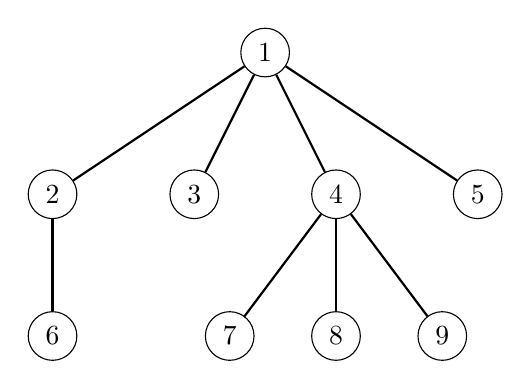
\begin{tikzpicture}[scale=0.9]
\node[draw, circle] (1) at (0,3) {$1$};
\node[draw, circle] (2) at (-3,1) {$2$};
\node[draw, circle] (3) at (-1,1) {$3$};
\node[draw, circle] (4) at (1,1) {$4$};
\node[draw, circle] (5) at (3,1) {$5$};
\node[draw, circle] (6) at (-3,-1) {$6$};
\node[draw, circle] (7) at (-0.5,-1) {$7$};
\node[draw, circle] (8) at (1,-1) {$8$};
\node[draw, circle] (9) at (2.5,-1) {$9$};

\path[draw,thick,-] (1) -- (2);
\path[draw,thick,-] (1) -- (3);
\path[draw,thick,-] (1) -- (4);
\path[draw,thick,-] (1) -- (5);
\path[draw,thick,-] (2) -- (6);
\path[draw,thick,-] (4) -- (7);
\path[draw,thick,-] (4) -- (8);
\path[draw,thick,-] (4) -- (9);
\end{tikzpicture}
\end{center}
pretraživanje u dubinu odvija se ovako:
\begin{center}
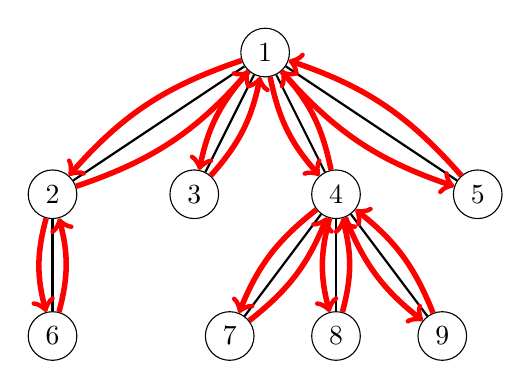
\begin{tikzpicture}[scale=0.9]
\node[draw, circle] (1) at (0,3) {$1$};
\node[draw, circle] (2) at (-3,1) {$2$};
\node[draw, circle] (3) at (-1,1) {$3$};
\node[draw, circle] (4) at (1,1) {$4$};
\node[draw, circle] (5) at (3,1) {$5$};
\node[draw, circle] (6) at (-3,-1) {$6$};
\node[draw, circle] (7) at (-0.5,-1) {$7$};
\node[draw, circle] (8) at (1,-1) {$8$};
\node[draw, circle] (9) at (2.5,-1) {$9$};

\path[draw,thick,-] (1) -- (2);
\path[draw,thick,-] (1) -- (3);
\path[draw,thick,-] (1) -- (4);
\path[draw,thick,-] (1) -- (5);
\path[draw,thick,-] (2) -- (6);
\path[draw,thick,-] (4) -- (7);
\path[draw,thick,-] (4) -- (8);
\path[draw,thick,-] (4) -- (9);


\path[draw=red,thick,->,line width=2pt] (1) edge [bend right=15] (2);
\path[draw=red,thick,->,line width=2pt] (2) edge [bend right=15] (6);
\path[draw=red,thick,->,line width=2pt] (6) edge [bend right=15] (2);
\path[draw=red,thick,->,line width=2pt] (2) edge [bend right=15] (1);
\path[draw=red,thick,->,line width=2pt] (1) edge [bend right=15] (3);
\path[draw=red,thick,->,line width=2pt] (3) edge [bend right=15] (1);
\path[draw=red,thick,->,line width=2pt] (1) edge [bend right=15] (4);
\path[draw=red,thick,->,line width=2pt] (4) edge [bend right=15] (7);
\path[draw=red,thick,->,line width=2pt] (7) edge [bend right=15] (4);
\path[draw=red,thick,->,line width=2pt] (4) edge [bend right=15] (8);
\path[draw=red,thick,->,line width=2pt] (8) edge [bend right=15] (4);
\path[draw=red,thick,->,line width=2pt] (4) edge [bend right=15] (9);
\path[draw=red,thick,->,line width=2pt] (9) edge [bend right=15] (4);
\path[draw=red,thick,->,line width=2pt] (4) edge [bend right=15] (1);
\path[draw=red,thick,->,line width=2pt] (1) edge [bend right=15] (5);
\path[draw=red,thick,->,line width=2pt] (5) edge [bend right=15] (1);

\end{tikzpicture}
\end{center}
Stoga je pripadni niz obilaska stabla sljedeći:
\begin{center}
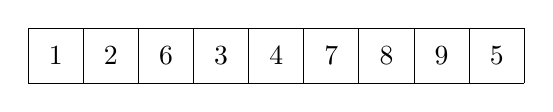
\begin{tikzpicture}[scale=0.7]
\draw (0,0) grid (9,1);

\node at (0.5,0.5) {$1$};
\node at (1.5,0.5) {$2$};
\node at (2.5,0.5) {$6$};
\node at (3.5,0.5) {$3$};
\node at (4.5,0.5) {$4$};
\node at (5.5,0.5) {$7$};
\node at (6.5,0.5) {$8$};
\node at (7.5,0.5) {$9$};
\node at (8.5,0.5) {$5$};
% 
% \footnotesize
% \node at (0.5,1.4) {$1$};
% \node at (1.5,1.4) {$2$};
% \node at (2.5,1.4) {$3$};
% \node at (3.5,1.4) {$4$};
% \node at (4.5,1.4) {$5$};
% \node at (5.5,1.4) {$6$};
% \node at (6.5,1.4) {$7$};
% \node at (7.5,1.4) {$8$};
% \node at (8.5,1.4) {$9$};
\end{tikzpicture}
\end{center}

\subsubsection{Upiti nad podstablima}

Svako podstablo stabla odgovara podnizu
niza obilaska stabla u kojem je
prvi element korijen tog podstabla.
Na primjer, sljedeći podniz sadrži
čvorove podstabla čvora $4$:
\begin{center}
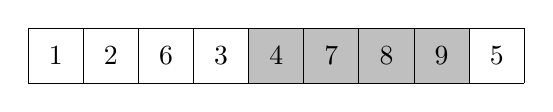
\begin{tikzpicture}[scale=0.7]
\fill[color=lightgray] (4,0) rectangle (8,1);
\draw (0,0) grid (9,1);

\node at (0.5,0.5) {$1$};
\node at (1.5,0.5) {$2$};
\node at (2.5,0.5) {$6$};
\node at (3.5,0.5) {$3$};
\node at (4.5,0.5) {$4$};
\node at (5.5,0.5) {$7$};
\node at (6.5,0.5) {$8$};
\node at (7.5,0.5) {$9$};
\node at (8.5,0.5) {$5$};
% 
% \footnotesize
% \node at (0.5,1.4) {$1$};
% \node at (1.5,1.4) {$2$};
% \node at (2.5,1.4) {$3$};
% \node at (3.5,1.4) {$4$};
% \node at (4.5,1.4) {$5$};
% \node at (5.5,1.4) {$6$};
% \node at (6.5,1.4) {$7$};
% \node at (7.5,1.4) {$8$};
% \node at (8.5,1.4) {$9$};
\end{tikzpicture}
\end{center}
Koristeći tu činjenicu, možemo efikasno obrađivati upite
koji se odnose na podstabla stabla.
Kao primjer promotrimo zadatak u kojem je svakom čvoru
pridružena vrijednost, a naš je zadatak podržati
sljedeće upite:
\begin{itemize}
\item ažuriraj vrijednost čvora
\item izračunaj sumu vrijednosti u podstablu čvora
\end{itemize}

Promotrimo sljedeće stablo u kojem su plavi brojevi
vrijednosti čvorova.
Na primjer, suma podstabla čvora $4$
iznosi $3+4+3+1=11$.

\begin{center}
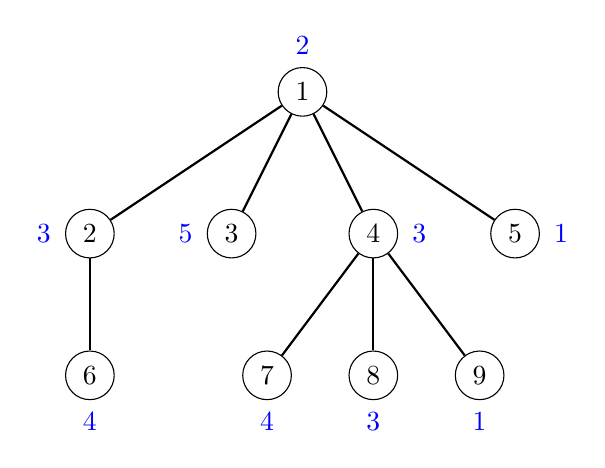
\begin{tikzpicture}[scale=0.9]
\node[draw, circle] (1) at (0,3) {$1$};
\node[draw, circle] (2) at (-3,1) {$2$};
\node[draw, circle] (3) at (-1,1) {$3$};
\node[draw, circle] (4) at (1,1) {$4$};
\node[draw, circle] (5) at (3,1) {$5$};
\node[draw, circle] (6) at (-3,-1) {$6$};
\node[draw, circle] (7) at (-0.5,-1) {$7$};
\node[draw, circle] (8) at (1,-1) {$8$};
\node[draw, circle] (9) at (2.5,-1) {$9$};

\path[draw,thick,-] (1) -- (2);
\path[draw,thick,-] (1) -- (3);
\path[draw,thick,-] (1) -- (4);
\path[draw,thick,-] (1) -- (5);
\path[draw,thick,-] (2) -- (6);
\path[draw,thick,-] (4) -- (7);
\path[draw,thick,-] (4) -- (8);
\path[draw,thick,-] (4) -- (9);

\node[color=blue] at (0,3+0.65) {2};
\node[color=blue] at (-3-0.65,1) {3};
\node[color=blue] at (-1-0.65,1) {5};
\node[color=blue] at (1+0.65,1) {3};
\node[color=blue] at (3+0.65,1) {1};
\node[color=blue] at (-3,-1-0.65) {4};
\node[color=blue] at (-0.5,-1-0.65) {4};
\node[color=blue] at (1,-1-0.65) {3};
\node[color=blue] at (2.5,-1-0.65) {1};
\end{tikzpicture}
\end{center}

Ideja je konstruirati niz obilaska stabla koji za svaki
čvor sadrži tri vrijednosti: identifikator čvora,
veličinu podstabla i vrijednost čvora.
Za gornje stablo taj je niz sljedeći:

\begin{center}
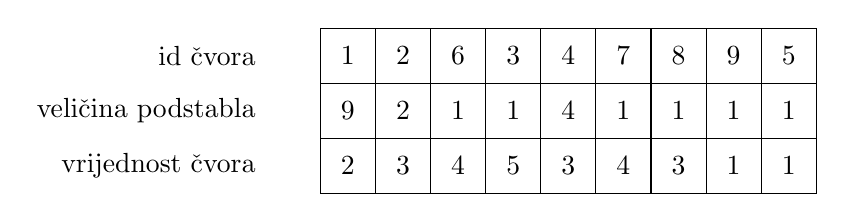
\begin{tikzpicture}[scale=0.7]
\draw (0,1) grid (9,-2);

\node[left] at (-1,0.5) {id čvora};
\node[left] at (-1,-0.5) {veličina podstabla};
\node[left] at (-1,-1.5) {vrijednost čvora};

\node at (0.5,0.5) {$1$};
\node at (1.5,0.5) {$2$};
\node at (2.5,0.5) {$6$};
\node at (3.5,0.5) {$3$};
\node at (4.5,0.5) {$4$};
\node at (5.5,0.5) {$7$};
\node at (6.5,0.5) {$8$};
\node at (7.5,0.5) {$9$};
\node at (8.5,0.5) {$5$};

\node at (0.5,-0.5) {$9$};
\node at (1.5,-0.5) {$2$};
\node at (2.5,-0.5) {$1$};
\node at (3.5,-0.5) {$1$};
\node at (4.5,-0.5) {$4$};
\node at (5.5,-0.5) {$1$};
\node at (6.5,-0.5) {$1$};
\node at (7.5,-0.5) {$1$};
\node at (8.5,-0.5) {$1$};

\node at (0.5,-1.5) {$2$};
\node at (1.5,-1.5) {$3$};
\node at (2.5,-1.5) {$4$};
\node at (3.5,-1.5) {$5$};
\node at (4.5,-1.5) {$3$};
\node at (5.5,-1.5) {$4$};
\node at (6.5,-1.5) {$3$};
\node at (7.5,-1.5) {$1$};
\node at (8.5,-1.5) {$1$};
% 
% \footnotesize
% \node at (0.5,1.4) {$1$};
% \node at (1.5,1.4) {$2$};
% \node at (2.5,1.4) {$3$};
% \node at (3.5,1.4) {$4$};
% \node at (4.5,1.4) {$5$};
% \node at (5.5,1.4) {$6$};
% \node at (6.5,1.4) {$7$};
% \node at (7.5,1.4) {$8$};
% \node at (8.5,1.4) {$9$};
\end{tikzpicture}
\end{center}

Pomoću tog niza možemo izračunati sumu vrijednosti
u bilo kojem podstablu tako da najprije odredimo veličinu podstabla,
a zatim vrijednosti pripadnih čvorova.
Na primjer, vrijednosti u podstablu čvora $4$
možemo pronaći ovako:

\begin{center}
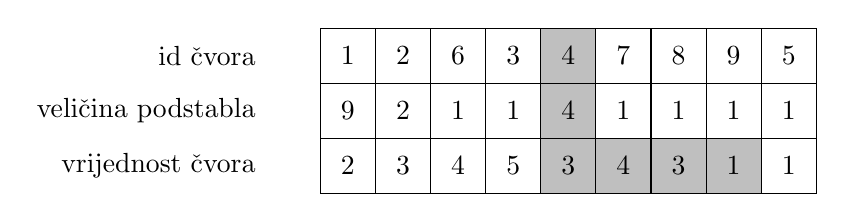
\begin{tikzpicture}[scale=0.7]
\fill[color=lightgray] (4,1) rectangle (5,0);
\fill[color=lightgray] (4,0) rectangle (5,-1);
\fill[color=lightgray] (4,-1) rectangle (8,-2);
\draw (0,1) grid (9,-2);

\node[left] at (-1,0.5) {id čvora};
\node[left] at (-1,-0.5) {veličina podstabla};
\node[left] at (-1,-1.5) {vrijednost čvora};

\node at (0.5,0.5) {$1$};
\node at (1.5,0.5) {$2$};
\node at (2.5,0.5) {$6$};
\node at (3.5,0.5) {$3$};
\node at (4.5,0.5) {$4$};
\node at (5.5,0.5) {$7$};
\node at (6.5,0.5) {$8$};
\node at (7.5,0.5) {$9$};
\node at (8.5,0.5) {$5$};

\node at (0.5,-0.5) {$9$};
\node at (1.5,-0.5) {$2$};
\node at (2.5,-0.5) {$1$};
\node at (3.5,-0.5) {$1$};
\node at (4.5,-0.5) {$4$};
\node at (5.5,-0.5) {$1$};
\node at (6.5,-0.5) {$1$};
\node at (7.5,-0.5) {$1$};
\node at (8.5,-0.5) {$1$};

\node at (0.5,-1.5) {$2$};
\node at (1.5,-1.5) {$3$};
\node at (2.5,-1.5) {$4$};
\node at (3.5,-1.5) {$5$};
\node at (4.5,-1.5) {$3$};
\node at (5.5,-1.5) {$4$};
\node at (6.5,-1.5) {$3$};
\node at (7.5,-1.5) {$1$};
\node at (8.5,-1.5) {$1$};
% 
% \footnotesize
% \node at (0.5,1.4) {$1$};
% \node at (1.5,1.4) {$2$};
% \node at (2.5,1.4) {$3$};
% \node at (3.5,1.4) {$4$};
% \node at (4.5,1.4) {$5$};
% \node at (5.5,1.4) {$6$};
% \node at (6.5,1.4) {$7$};
% \node at (7.5,1.4) {$8$};
% \node at (8.5,1.4) {$9$};
\end{tikzpicture}
\end{center}

Za efikasno odgovaranje na upite
dovoljno je vrijednosti čvorova pohraniti
u binarno indeksirano ili segmentno stablo.
Nakon toga možemo i ažurirati vrijednost
i izračunati sumu vrijednosti u $O(\log n)$ vremenu.

\subsubsection{Upiti nad putovima}

Pomoću niza obilaska stabla možemo također efikasno
računati sume vrijednosti na
putovima od korijena do bilo kojeg
čvora stabla.
Promotrimo zadatak u kojem trebamo
podržati sljedeće upite:
\begin{itemize}
\item promijeni vrijednost čvora
\item izračunaj sumu vrijednosti na putu od
korijena do čvora
\end{itemize}

Na primjer, u sljedećem stablu
suma vrijednosti od korijena do čvora 7 iznosi
$4+5+5=14$:

\begin{center}
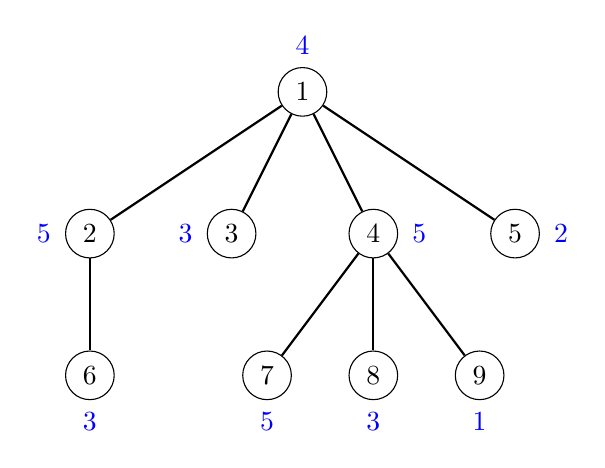
\begin{tikzpicture}[scale=0.9]
\node[draw, circle] (1) at (0,3) {$1$};
\node[draw, circle] (2) at (-3,1) {$2$};
\node[draw, circle] (3) at (-1,1) {$3$};
\node[draw, circle] (4) at (1,1) {$4$};
\node[draw, circle] (5) at (3,1) {$5$};
\node[draw, circle] (6) at (-3,-1) {$6$};
\node[draw, circle] (7) at (-0.5,-1) {$7$};
\node[draw, circle] (8) at (1,-1) {$8$};
\node[draw, circle] (9) at (2.5,-1) {$9$};

\path[draw,thick,-] (1) -- (2);
\path[draw,thick,-] (1) -- (3);
\path[draw,thick,-] (1) -- (4);
\path[draw,thick,-] (1) -- (5);
\path[draw,thick,-] (2) -- (6);
\path[draw,thick,-] (4) -- (7);
\path[draw,thick,-] (4) -- (8);
\path[draw,thick,-] (4) -- (9);

\node[color=blue] at (0,3+0.65) {4};
\node[color=blue] at (-3-0.65,1) {5};
\node[color=blue] at (-1-0.65,1) {3};
\node[color=blue] at (1+0.65,1) {5};
\node[color=blue] at (3+0.65,1) {2};
\node[color=blue] at (-3,-1-0.65) {3};
\node[color=blue] at (-0.5,-1-0.65) {5};
\node[color=blue] at (1,-1-0.65) {3};
\node[color=blue] at (2.5,-1-0.65) {1};
\end{tikzpicture}
\end{center}

Ovaj zadatak možemo riješiti kao i prije,
ali sada je svaka vrijednost u posljednjem redu niza suma vrijednosti
na putu od korijena do tog čvora.
Na primjer, sljedeći niz odgovara gornjem stablu:
\begin{center}
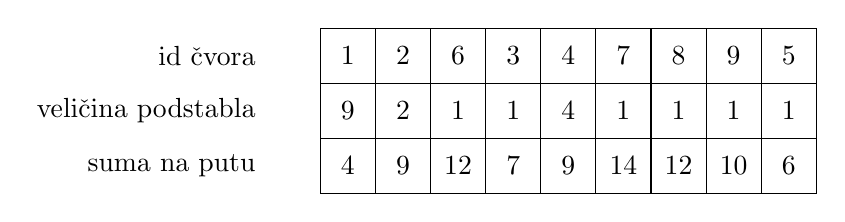
\begin{tikzpicture}[scale=0.7]
\draw (0,1) grid (9,-2);

\node[left] at (-1,0.5) {id čvora};
\node[left] at (-1,-0.5) {veličina podstabla};
\node[left] at (-1,-1.5) {suma na putu};

\node at (0.5,0.5) {$1$};
\node at (1.5,0.5) {$2$};
\node at (2.5,0.5) {$6$};
\node at (3.5,0.5) {$3$};
\node at (4.5,0.5) {$4$};
\node at (5.5,0.5) {$7$};
\node at (6.5,0.5) {$8$};
\node at (7.5,0.5) {$9$};
\node at (8.5,0.5) {$5$};

\node at (0.5,-0.5) {$9$};
\node at (1.5,-0.5) {$2$};
\node at (2.5,-0.5) {$1$};
\node at (3.5,-0.5) {$1$};
\node at (4.5,-0.5) {$4$};
\node at (5.5,-0.5) {$1$};
\node at (6.5,-0.5) {$1$};
\node at (7.5,-0.5) {$1$};
\node at (8.5,-0.5) {$1$};

\node at (0.5,-1.5) {$4$};
\node at (1.5,-1.5) {$9$};
\node at (2.5,-1.5) {$12$};
\node at (3.5,-1.5) {$7$};
\node at (4.5,-1.5) {$9$};
\node at (5.5,-1.5) {$14$};
\node at (6.5,-1.5) {$12$};
\node at (7.5,-1.5) {$10$};
\node at (8.5,-1.5) {$6$};
\end{tikzpicture}
\end{center}

Kada se vrijednost čvora poveća za $x$,
sume svih čvorova u njegovu podstablu povećavaju se za $x$.
Na primjer, ako se vrijednost čvora 4 poveća za 1,
niz se mijenja ovako:

\begin{center}
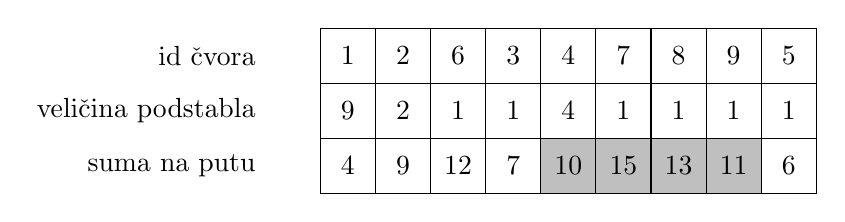
\begin{tikzpicture}[scale=0.7]
\fill[color=lightgray] (4,-1) rectangle (8,-2);
\draw (0,1) grid (9,-2);

\node[left] at (-1,0.5) {id čvora};
\node[left] at (-1,-0.5) {veličina podstabla};
\node[left] at (-1,-1.5) {suma na putu};

\node at (0.5,0.5) {$1$};
\node at (1.5,0.5) {$2$};
\node at (2.5,0.5) {$6$};
\node at (3.5,0.5) {$3$};
\node at (4.5,0.5) {$4$};
\node at (5.5,0.5) {$7$};
\node at (6.5,0.5) {$8$};
\node at (7.5,0.5) {$9$};
\node at (8.5,0.5) {$5$};

\node at (0.5,-0.5) {$9$};
\node at (1.5,-0.5) {$2$};
\node at (2.5,-0.5) {$1$};
\node at (3.5,-0.5) {$1$};
\node at (4.5,-0.5) {$4$};
\node at (5.5,-0.5) {$1$};
\node at (6.5,-0.5) {$1$};
\node at (7.5,-0.5) {$1$};
\node at (8.5,-0.5) {$1$};

\node at (0.5,-1.5) {$4$};
\node at (1.5,-1.5) {$9$};
\node at (2.5,-1.5) {$12$};
\node at (3.5,-1.5) {$7$};
\node at (4.5,-1.5) {$10$};
\node at (5.5,-1.5) {$15$};
\node at (6.5,-1.5) {$13$};
\node at (7.5,-1.5) {$11$};
\node at (8.5,-1.5) {$6$};
\end{tikzpicture}
\end{center}

Dakle, da bismo podržali obje operacije,
moramo moći povećati sve vrijednosti
u intervalu i dohvatiti pojedinačnu vrijednost.
To se može učiniti u $O(\log n)$ vremenu
pomoću binarno indeksiranog
ili segmentnog stabla (vidi poglavlje 9.4).

\section{Najniži zajednički predak}

\index{najniži zajednički predak}

\key{Najniži zajednički predak}
dvaju čvorova korijenskog stabla je najniži čvor
čije podstablo sadrži oba ta čvora.
Tipičan je zadatak efikasno obraditi
upite koji traže najnižeg
zajedničkog pretka dvaju čvorova.

Na primjer, u sljedećem stablu
najniži zajednički predak čvorova 5 i 8
je čvor 2:
\begin{center}
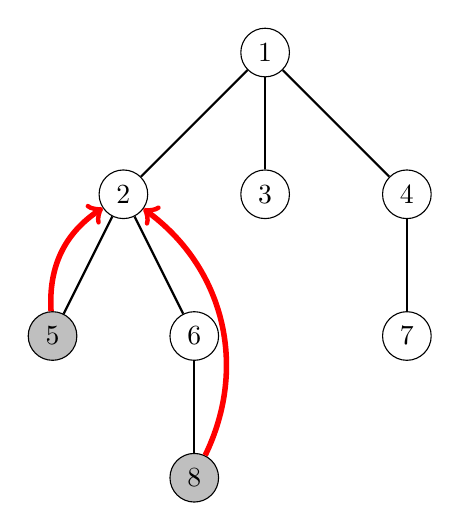
\begin{tikzpicture}[scale=0.9]
\node[draw, circle] (1) at (0,3) {$1$};
\node[draw, circle] (2) at (2,1) {$4$};
\node[draw, circle] (3) at (-2,1) {$2$};
\node[draw, circle] (4) at (0,1) {$3$};
\node[draw, circle] (5) at (2,-1) {$7$};
\node[draw, circle, fill=lightgray] (6) at (-3,-1) {$5$};
\node[draw, circle] (7) at (-1,-1) {$6$};
\node[draw, circle, fill=lightgray] (8) at (-1,-3) {$8$};
\path[draw,thick,-] (1) -- (2);
\path[draw,thick,-] (1) -- (3);
\path[draw,thick,-] (1) -- (4);
\path[draw,thick,-] (2) -- (5);
\path[draw,thick,-] (3) -- (6);
\path[draw,thick,-] (3) -- (7);
\path[draw,thick,-] (7) -- (8);

\path[draw=red,thick,->,line width=2pt] (6) edge [bend left] (3);
\path[draw=red,thick,->,line width=2pt] (8) edge [bend right=40] (3);
\end{tikzpicture}
\end{center}

U nastavku razmatramo dvije efikasne tehnike za
pronalaženje najnižeg zajedničkog pretka dvaju čvorova.

\subsubsection{Metoda 1}

Jedan je način rješavanja zadatka iskoristiti činjenicu
da možemo efikasno pronaći $k$-tog
pretka bilo kojeg čvora u stablu.
Pomoću toga zadatak pronalaženja
najnižeg zajedničkog pretka možemo podijeliti na dva dijela.

Koristimo dva pokazivača koji na početku pokazuju na
dva čvora čijeg najnižeg zajedničkog pretka trebamo pronaći.
Najprije jedan od pokazivača pomičemo prema gore
tako da oba pokazivača pokazuju na čvorove na istoj razini.

U ovom primjeru pomičemo drugi pokazivač jednu
razinu prema gore tako da pokazuje na čvor 6,
koji je na istoj razini kao čvor 5:

\begin{center}
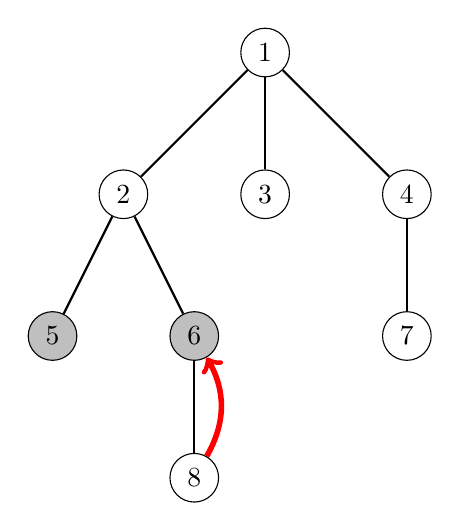
\begin{tikzpicture}[scale=0.9]
\node[draw, circle] (1) at (0,3) {$1$};
\node[draw, circle] (2) at (2,1) {$4$};
\node[draw, circle] (3) at (-2,1) {$2$};
\node[draw, circle] (4) at (0,1) {$3$};
\node[draw, circle] (5) at (2,-1) {$7$};
\node[draw, circle,fill=lightgray] (6) at (-3,-1) {$5$};
\node[draw, circle,fill=lightgray] (7) at (-1,-1) {$6$};
\node[draw, circle] (8) at (-1,-3) {$8$};
\path[draw,thick,-] (1) -- (2);
\path[draw,thick,-] (1) -- (3);
\path[draw,thick,-] (1) -- (4);
\path[draw,thick,-] (2) -- (5);
\path[draw,thick,-] (3) -- (6);
\path[draw,thick,-] (3) -- (7);
\path[draw,thick,-] (7) -- (8);

\path[draw=red,thick,->,line width=2pt] (8) edge [bend right] (7);
\end{tikzpicture}
\end{center}

Nakon toga određujemo najmanji broj koraka
potreban da oba pokazivača pomaknemo prema gore tako da
pokazuju na isti čvor.
Čvor na koji pokazivači tada pokazuju
najniži je zajednički predak.

U ovom primjeru dovoljno je oba pokazivača pomaknuti
jedan korak prema gore do čvora 2,
koji je najniži zajednički predak:

\begin{center}
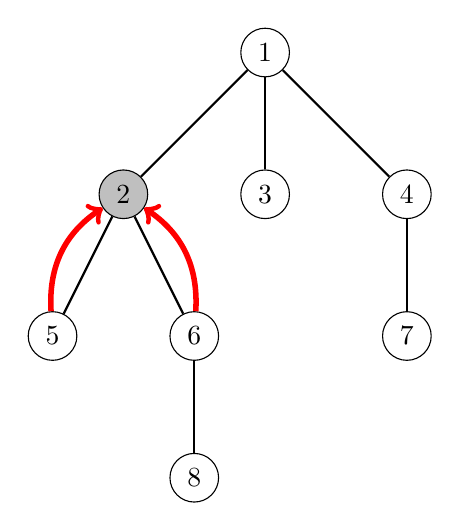
\begin{tikzpicture}[scale=0.9]
\node[draw, circle] (1) at (0,3) {$1$};
\node[draw, circle] (2) at (2,1) {$4$};
\node[draw, circle,fill=lightgray] (3) at (-2,1) {$2$};
\node[draw, circle] (4) at (0,1) {$3$};
\node[draw, circle] (5) at (2,-1) {$7$};
\node[draw, circle] (6) at (-3,-1) {$5$};
\node[draw, circle] (7) at (-1,-1) {$6$};
\node[draw, circle] (8) at (-1,-3) {$8$};
\path[draw,thick,-] (1) -- (2);
\path[draw,thick,-] (1) -- (3);
\path[draw,thick,-] (1) -- (4);
\path[draw,thick,-] (2) -- (5);
\path[draw,thick,-] (3) -- (6);
\path[draw,thick,-] (3) -- (7);
\path[draw,thick,-] (7) -- (8);

\path[draw=red,thick,->,line width=2pt] (6) edge [bend left] (3);
\path[draw=red,thick,->,line width=2pt] (7) edge [bend right] (3);
\end{tikzpicture}
\end{center}

Budući da se oba dijela algoritma mogu izvesti u
$O(\log n)$ vremenu uz unaprijed izračunate podatke,
najnižeg zajedničkog pretka bilo kojih dvaju
čvorova možemo pronaći u $O(\log n)$ vremenu.

\subsubsection{Metoda 2}

Drugi način rješavanja zadatka temelji se na
nizu obilaska stabla\footnote{Ovaj algoritam za najnižeg zajedničkog pretka predstavljen je u \cite{ben00}.
Ta se tehnika ponekad naziva \index{Eulerova tehnika obilaska}
\key{Eulerova tehnika obilaska} \cite{tar84}.}.
I ovdje je ideja obići čvorove
pretraživanjem u dubinu:

\begin{center}
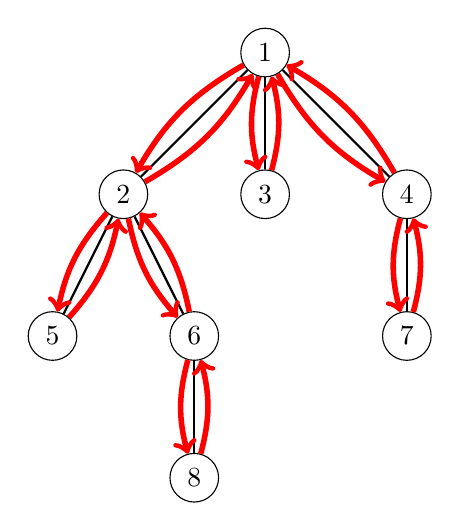
\begin{tikzpicture}[scale=0.9]
\node[draw, circle] (1) at (0,3) {$1$};
\node[draw, circle] (2) at (2,1) {$4$};
\node[draw, circle] (3) at (-2,1) {$2$};
\node[draw, circle] (4) at (0,1) {$3$};
\node[draw, circle] (5) at (2,-1) {$7$};
\node[draw, circle] (6) at (-3,-1) {$5$};
\node[draw, circle] (7) at (-1,-1) {$6$};
\node[draw, circle] (8) at (-1,-3) {$8$};
\path[draw,thick,-] (1) -- (2);
\path[draw,thick,-] (1) -- (3);
\path[draw,thick,-] (1) -- (4);
\path[draw,thick,-] (2) -- (5);
\path[draw,thick,-] (3) -- (6);
\path[draw,thick,-] (3) -- (7);
\path[draw,thick,-] (7) -- (8);

\path[draw=red,thick,->,line width=2pt] (1) edge [bend right=15] (3);
\path[draw=red,thick,->,line width=2pt] (3) edge [bend right=15] (6);
\path[draw=red,thick,->,line width=2pt] (6) edge [bend right=15] (3);
\path[draw=red,thick,->,line width=2pt] (3) edge [bend right=15] (7);
\path[draw=red,thick,->,line width=2pt] (7) edge [bend right=15] (8);
\path[draw=red,thick,->,line width=2pt] (8) edge [bend right=15] (7);
\path[draw=red,thick,->,line width=2pt] (7) edge [bend right=15] (3);
\path[draw=red,thick,->,line width=2pt] (3) edge [bend right=15] (1);
\path[draw=red,thick,->,line width=2pt] (1) edge [bend right=15] (4);
\path[draw=red,thick,->,line width=2pt] (4) edge [bend right=15] (1);
\path[draw=red,thick,->,line width=2pt] (1) edge [bend right=15] (2);
\path[draw=red,thick,->,line width=2pt] (2) edge [bend right=15] (5);
\path[draw=red,thick,->,line width=2pt] (5) edge [bend right=15] (2);
\path[draw=red,thick,->,line width=2pt] (2) edge [bend right=15] (1);
\end{tikzpicture}
\end{center}

Međutim, sada koristimo drugačiji niz
obilaska stabla nego prije:
čvor dodajemo u niz \emph{svaki put}
kad pretraživanje u dubinu prođe kroz njega,
a ne samo pri prvom posjetu.
Stoga se čvor koji ima $k$ djece pojavljuje $k+1$ puta
u nizu, pa niz ukupno sadrži $2n-1$
čvorova.

U nizu pohranjujemo dvije vrijednosti:
identifikator čvora i dubinu 
čvora u stablu.
Sljedeći niz odgovara gornjem stablu:

\begin{center}
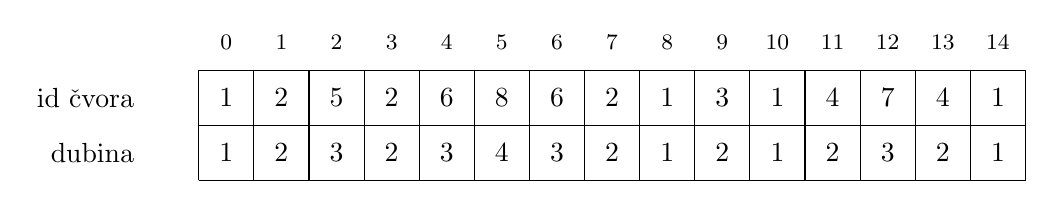
\begin{tikzpicture}[scale=0.7]

\node[left] at (-1,1.5) {id čvora};
\node[left] at (-1,0.5) {dubina};

\draw (0,1) grid (15,2);
\node at (0.5,1.5) {$1$};
\node at (1.5,1.5) {$2$};
\node at (2.5,1.5) {$5$};
\node at (3.5,1.5) {$2$};
\node at (4.5,1.5) {$6$};
\node at (5.5,1.5) {$8$};
\node at (6.5,1.5) {$6$};
\node at (7.5,1.5) {$2$};
\node at (8.5,1.5) {$1$};
\node at (9.5,1.5) {$3$};
\node at (10.5,1.5) {$1$};
\node at (11.5,1.5) {$4$};
\node at (12.5,1.5) {$7$};
\node at (13.5,1.5) {$4$};
\node at (14.5,1.5) {$1$};

\draw (0,0) grid (15,1);
\node at (0.5,0.5) {$1$};
\node at (1.5,0.5) {$2$};
\node at (2.5,0.5) {$3$};
\node at (3.5,0.5) {$2$};
\node at (4.5,0.5) {$3$};
\node at (5.5,0.5) {$4$};
\node at (6.5,0.5) {$3$};
\node at (7.5,0.5) {$2$};
\node at (8.5,0.5) {$1$};
\node at (9.5,0.5) {$2$};
\node at (10.5,0.5) {$1$};
\node at (11.5,0.5) {$2$};
\node at (12.5,0.5) {$3$};
\node at (13.5,0.5) {$2$};
\node at (14.5,0.5) {$1$};

\footnotesize
\node at (0.5,2.5) {$0$};
\node at (1.5,2.5) {$1$};
\node at (2.5,2.5) {$2$};
\node at (3.5,2.5) {$3$};
\node at (4.5,2.5) {$4$};
\node at (5.5,2.5) {$5$};
\node at (6.5,2.5) {$6$};
\node at (7.5,2.5) {$7$};
\node at (8.5,2.5) {$8$};
\node at (9.5,2.5) {$9$};
\node at (10.5,2.5) {$10$};
\node at (11.5,2.5) {$11$};
\node at (12.5,2.5) {$12$};
\node at (13.5,2.5) {$13$};
\node at (14.5,2.5) {$14$};
\end{tikzpicture}
\end{center}

Sada najnižeg zajedničkog pretka
čvorova $a$ i $b$ možemo pronaći tako da pronađemo čvor s \emph{najmanjom} dubinom
između čvorova $a$ i $b$ u nizu.
Na primjer, najnižeg zajedničkog pretka čvorova $5$ i $8$
možemo pronaći ovako:

\begin{center}
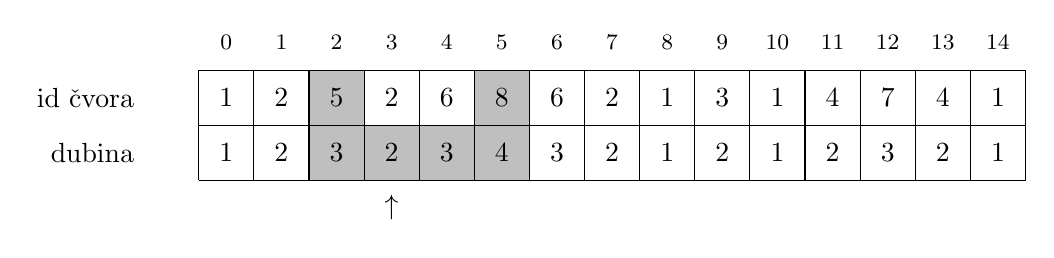
\begin{tikzpicture}[scale=0.7]

\node[left] at (-1,1.5) {id čvora};
\node[left] at (-1,0.5) {dubina};

\fill[color=lightgray] (2,1) rectangle (3,2);
\fill[color=lightgray] (5,1) rectangle (6,2);
\fill[color=lightgray] (2,0) rectangle (6,1);

\node at (3.5,-0.5) {$\uparrow$};

\draw (0,1) grid (15,2);
\node at (0.5,1.5) {$1$};
\node at (1.5,1.5) {$2$};
\node at (2.5,1.5) {$5$};
\node at (3.5,1.5) {$2$};
\node at (4.5,1.5) {$6$};
\node at (5.5,1.5) {$8$};
\node at (6.5,1.5) {$6$};
\node at (7.5,1.5) {$2$};
\node at (8.5,1.5) {$1$};
\node at (9.5,1.5) {$3$};
\node at (10.5,1.5) {$1$};
\node at (11.5,1.5) {$4$};
\node at (12.5,1.5) {$7$};
\node at (13.5,1.5) {$4$};
\node at (14.5,1.5) {$1$};


\draw (0,0) grid (15,1);
\node at (0.5,0.5) {$1$};
\node at (1.5,0.5) {$2$};
\node at (2.5,0.5) {$3$};
\node at (3.5,0.5) {$2$};
\node at (4.5,0.5) {$3$};
\node at (5.5,0.5) {$4$};
\node at (6.5,0.5) {$3$};
\node at (7.5,0.5) {$2$};
\node at (8.5,0.5) {$1$};
\node at (9.5,0.5) {$2$};
\node at (10.5,0.5) {$1$};
\node at (11.5,0.5) {$2$};
\node at (12.5,0.5) {$3$};
\node at (13.5,0.5) {$2$};
\node at (14.5,0.5) {$1$};

\footnotesize
\node at (0.5,2.5) {$0$};
\node at (1.5,2.5) {$1$};
\node at (2.5,2.5) {$2$};
\node at (3.5,2.5) {$3$};
\node at (4.5,2.5) {$4$};
\node at (5.5,2.5) {$5$};
\node at (6.5,2.5) {$6$};
\node at (7.5,2.5) {$7$};
\node at (8.5,2.5) {$8$};
\node at (9.5,2.5) {$9$};
\node at (10.5,2.5) {$10$};
\node at (11.5,2.5) {$11$};
\node at (12.5,2.5) {$12$};
\node at (13.5,2.5) {$13$};
\node at (14.5,2.5) {$14$};
\end{tikzpicture}
\end{center}

Čvor 5 nalazi se na poziciji 2, čvor 8 na poziciji 5,
a čvor s najmanjom dubinom između
pozicija $2 \ldots 5$ je čvor 2 na poziciji 3,
čija je dubina 2.
Dakle, najniži zajednički predak
čvorova 5 i 8 je čvor 2.

Dakle, za pronalaženje najnižeg zajedničkog pretka
dvaju čvorova dovoljno je obraditi upit
za minimum nad intervalom.
Budući da je niz statičan,
takve upite možemo obraditi u $O(1)$ vremenu
nakon predobrade u $O(n \log n)$ vremenu.

\subsubsection{Udaljenosti čvorova}

Udaljenost između čvorova $a$ i $b$
jednaka je duljini puta od $a$ do $b$.
Pokazuje se da se zadatak računanja
udaljenosti između čvorova svodi na
pronalaženje njihova najnižeg zajedničkog pretka.

Najprije stablo proizvoljno ukorijenimo.
Nakon toga udaljenost čvorova $a$ i $b$
možemo izračunati pomoću formule
\[\texttt{dubina}(a)+\texttt{dubina}(b)-2 \cdot \texttt{dubina}(c),\]
gdje je $c$ najniži zajednički predak čvorova $a$ i $b$,
a $\texttt{dubina}(s)$ označava dubinu čvora $s$.
Na primjer, promotrimo udaljenost čvorova 5 i 8:
\begin{center}
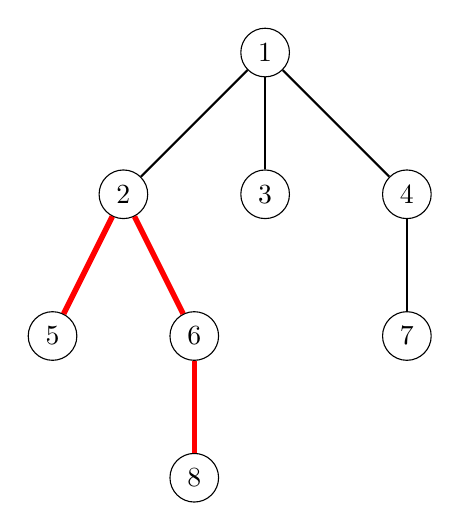
\begin{tikzpicture}[scale=0.9]
\node[draw, circle] (1) at (0,3) {$1$};
\node[draw, circle] (2) at (2,1) {$4$};
\node[draw, circle] (3) at (-2,1) {$2$};
\node[draw, circle] (4) at (0,1) {$3$};
\node[draw, circle] (5) at (2,-1) {$7$};
\node[draw, circle] (6) at (-3,-1) {$5$};
\node[draw, circle] (7) at (-1,-1) {$6$};
\node[draw, circle] (8) at (-1,-3) {$8$};
\path[draw,thick,-] (1) -- (2);
\path[draw,thick,-] (1) -- (3);
\path[draw,thick,-] (1) -- (4);
\path[draw,thick,-] (2) -- (5);
\path[draw,thick,-] (3) -- (6);
\path[draw,thick,-] (3) -- (7);
\path[draw,thick,-] (7) -- (8);

\path[draw=red,thick,-,line width=2pt] (8) -- node[font=\small] {} (7);
\path[draw=red,thick,-,line width=2pt] (7) -- node[font=\small] {} (3);
\path[draw=red,thick,-,line width=2pt] (6) -- node[font=\small] {} (3);
\end{tikzpicture}
\end{center}

Najniži zajednički predak čvorova 5 i 8 je čvor 2.
Dubine čvorova su
$\texttt{dubina}(5)=3$, $\texttt{dubina}(8)=4$ i $\texttt{dubina}(2)=2$,
pa je udaljenost između čvorova 5 i 8 jednaka
$3+4-2\cdot2=3$.

\section{Offline algoritmi}

Do sada smo razmatrali \emph{online} algoritme
za upite nad stablom.
Ti algoritmi mogu obrađivati
upite jedan za drugim tako da se
na svaki upit odgovori prije primanja sljedećeg upita.

Međutim, u mnogim zadacima online
svojstvo nije nužno.
U ovom se poglavlju usredotočujemo na \emph{offline} algoritme.
Tim je algoritmima zadan skup upita na koje se
može odgovoriti bilo kojim redoslijedom.
Često je lakše osmisliti offline algoritam
nego online algoritam.

\subsubsection{Spajanje struktura podataka}

Jedan način konstrukcije offline algoritma
jest izvesti obilazak stabla u dubinu
i održavati strukture podataka u čvorovima.
U svakom čvoru $s$ stvaramo strukturu podataka
$\texttt{d}[s]$ koja se temelji na
strukturama podataka djece čvora $s$.
Zatim se, pomoću te strukture podataka,
obrađuju svi upiti vezani uz $s$.

Kao primjer promotrimo sljedeći zadatak:
zadano nam je stablo u kojem svaki čvor ima neku vrijednost.
Naš je zadatak obraditi upite oblika
''izračunaj broj čvorova s vrijednošću $x$
u podstablu čvora $s$''.
Na primjer, u sljedećem stablu
podstablo čvora $4$ sadrži dva čvora
čija je vrijednost 3.

\begin{center}
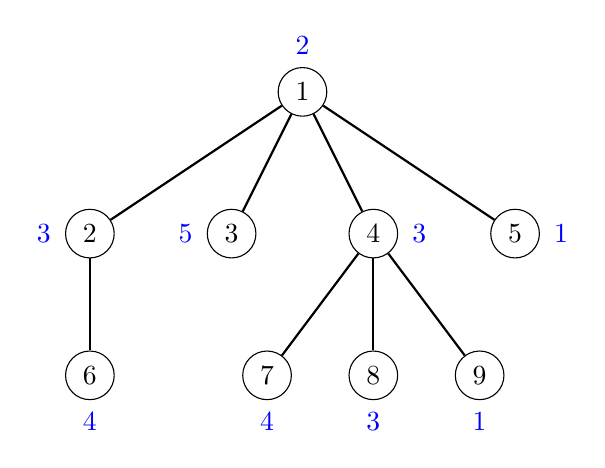
\begin{tikzpicture}[scale=0.9]
\node[draw, circle] (1) at (0,3) {$1$};
\node[draw, circle] (2) at (-3,1) {$2$};
\node[draw, circle] (3) at (-1,1) {$3$};
\node[draw, circle] (4) at (1,1) {$4$};
\node[draw, circle] (5) at (3,1) {$5$};
\node[draw, circle] (6) at (-3,-1) {$6$};
\node[draw, circle] (7) at (-0.5,-1) {$7$};
\node[draw, circle] (8) at (1,-1) {$8$};
\node[draw, circle] (9) at (2.5,-1) {$9$};

\path[draw,thick,-] (1) -- (2);
\path[draw,thick,-] (1) -- (3);
\path[draw,thick,-] (1) -- (4);
\path[draw,thick,-] (1) -- (5);
\path[draw,thick,-] (2) -- (6);
\path[draw,thick,-] (4) -- (7);
\path[draw,thick,-] (4) -- (8);
\path[draw,thick,-] (4) -- (9);

\node[color=blue] at (0,3+0.65) {2};
\node[color=blue] at (-3-0.65,1) {3};
\node[color=blue] at (-1-0.65,1) {5};
\node[color=blue] at (1+0.65,1) {3};
\node[color=blue] at (3+0.65,1) {1};
\node[color=blue] at (-3,-1-0.65) {4};
\node[color=blue] at (-0.5,-1-0.65) {4};
\node[color=blue] at (1,-1-0.65) {3};
\node[color=blue] at (2.5,-1-0.65) {1};
\end{tikzpicture}
\end{center}

U ovom zadatku za odgovaranje na upite
možemo koristiti mape.
Na primjer, mape za čvor 4 i
njegovu djecu su sljedeće:

\begin{center}
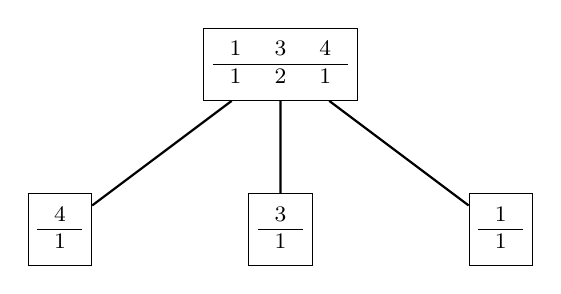
\begin{tikzpicture}[scale=0.7]

\node[draw, rectangle] (a) at (4,5.5)
{
\footnotesize
\begin{tabular}{rrr}
4 \\
\hline
1 \\
\end{tabular}};

\node[draw, rectangle] (b) at (8,5.5)
{
\footnotesize
\begin{tabular}{rrr}
3 \\
\hline
1 \\
\end{tabular}};


\node[draw, rectangle] (c) at (12,5.5)
{
\footnotesize
\begin{tabular}{rr}
1 \\
\hline
1 \\
\end{tabular}};

\node[draw, rectangle] (d) at (8,8.5)
{
\footnotesize
\begin{tabular}{rrr}
1 & 3 & 4 \\
\hline
1 & 2 & 1 \\
\end{tabular}};
\path[draw,thick,-] (a) -- (d);
\path[draw,thick,-] (b) -- (d);
\path[draw,thick,-] (c) -- (d);
\end{tikzpicture}
\end{center}

Ako takvu strukturu podataka stvorimo za svaki čvor,
lako možemo obraditi sve zadane upite
jer sve upite vezane uz neki čvor
možemo obraditi odmah nakon što stvorimo njegovu
strukturu podataka. Na primjer, gornja
mapa za čvor 4
govori nam da njegovo podstablo
sadrži dva čvora čija je vrijednost 3.

Međutim, stvaranje svih struktura podataka
od nule bilo bi presporo.
Umjesto toga, u svakom čvoru $s$
stvaramo početnu strukturu podataka $\texttt{d}[s]$ 
koja sadrži samo vrijednost čvora $s$.
Nakon toga prolazimo kroz djecu čvora $s$ i
\emph{spajamo} $\texttt{d}[s]$ sa
svim strukturama podataka
$\texttt{d}[u]$ gdje je $u$ dijete čvora $s$.

Na primjer, u gornjem stablu mapa
za čvor $4$ nastaje spajanjem sljedećih mapa:

\begin{center}
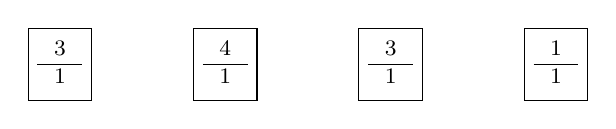
\begin{tikzpicture}[scale=0.7]

\node[draw, rectangle] (a) at (4,5.5)
{
\footnotesize
\begin{tabular}{rrr}
4 \\
\hline
1 \\
\end{tabular}};

\node[draw, rectangle] (b) at (7,5.5)
{
\footnotesize
\begin{tabular}{rrr}
3 \\
\hline
1 \\
\end{tabular}};

\node[draw, rectangle] (c) at (10,5.5)
{
\footnotesize
\begin{tabular}{rr}
1 \\
\hline
1 \\
\end{tabular}};

\node[draw, rectangle] (d) at (1,5.5)
{
\footnotesize
\begin{tabular}{rr}
3 \\
\hline
1 \\
\end{tabular}};

\end{tikzpicture}
\end{center}

Ovdje je prva mapa početna struktura podataka
za čvor 4,
a preostale tri mape odgovaraju čvorovima 7, 8 i 9.

Spajanje u čvoru $s$ možemo izvesti ovako:
prolazimo kroz djecu čvora $s$
i u svakom djetetu $u$ spajamo $\texttt{d}[s]$
i $\texttt{d}[u]$.
Sadržaj uvijek kopiramo iz $\texttt{d}[u]$
u $\texttt{d}[s]$.
Međutim, prije toga \emph{zamijenimo}
sadržaje struktura $\texttt{d}[s]$ i $\texttt{d}[u]$
ako je $\texttt{d}[s]$ manja od $\texttt{d}[u]$.
Na taj se način svaka vrijednost tijekom obilaska stabla
kopira samo $O(\log n)$ puta,
čime osiguravamo da je algoritam efikasan.

Za efikasnu zamjenu sadržaja dviju struktura podataka $a$ i $b$
možemo jednostavno upotrijebiti sljedeći kod:
\begin{lstlisting}
swap(a,b);
\end{lstlisting}
Zajamčeno je da gornji kod radi u konstantnom vremenu
kada su $a$ i $b$ strukture podataka iz standardne biblioteke jezika C++.

\subsubsection{Najniži zajednički preci}

Postoji i offline algoritam
za obradu skupa
upita o najnižem zajedničkom pretku\footnote{Ovaj je
algoritam objavio R. E. Tarjan 1979. godine \cite{tar79}.}.
Algoritam se temelji na strukturi podataka union-find
(vidi poglavlje 15.2), a njegova je prednost
to što ga je lakše implementirati od
algoritama razmatranih ranije u ovom poglavlju.

Algoritmu je kao ulaz zadan skup parova čvorova
te za svaki takav par određuje
najnižeg zajedničkog pretka tih čvorova.
Algoritam izvodi obilazak stabla u dubinu
i održava disjunktne skupove čvorova.
Na početku svaki čvor pripada zasebnom skupu.
Za svaki skup pamtimo i najviši čvor u
stablu koji pripada tom skupu.

Kada algoritam posjeti čvor $x$,
prolazi kroz sve čvorove $y$ za koje
treba pronaći najnižeg zajedničkog pretka
čvorova $x$ i $y$.
Ako je $y$ već posjećen,
algoritam javlja da je 
najniži zajednički predak čvorova $x$ i $y$
najviši čvor u skupu čvora $y$.
Zatim, nakon obrade čvora $x$,
algoritam spaja skupove čvora $x$ i njegova roditelja.

Na primjer, pretpostavimo da želimo pronaći najniže
zajedničke pretke parova čvorova $(5,8)$
i $(2,7)$ u sljedećem stablu:
\begin{center}
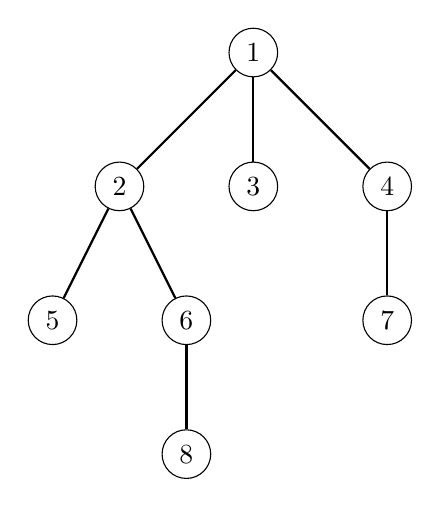
\begin{tikzpicture}[scale=0.85]
\node[draw, circle] (1) at (0,3) {$1$};
\node[draw, circle] (2) at (2,1) {$4$};
\node[draw, circle] (3) at (-2,1) {$2$};
\node[draw, circle] (4) at (0,1) {$3$};
\node[draw, circle] (5) at (2,-1) {$7$};
\node[draw, circle] (6) at (-3,-1) {$5$};
\node[draw, circle] (7) at (-1,-1) {$6$};
\node[draw, circle] (8) at (-1,-3) {$8$};
\path[draw,thick,-] (1) -- (2);
\path[draw,thick,-] (1) -- (3);
\path[draw,thick,-] (1) -- (4);
\path[draw,thick,-] (2) -- (5);
\path[draw,thick,-] (3) -- (6);
\path[draw,thick,-] (3) -- (7);
\path[draw,thick,-] (7) -- (8);
\end{tikzpicture}
\end{center}

U sljedećim stablima sivi čvorovi označavaju posjećene čvorove,
a isprekidano označene skupine čvorova pripadaju istom skupu.
Kada algoritam posjeti čvor 8, uočava da je
čvor 5 već posjećen i da je najviši čvor
u njegovu skupu 2. Dakle, najniži zajednički predak
čvorova 5 i 8 je 2:
\begin{center}
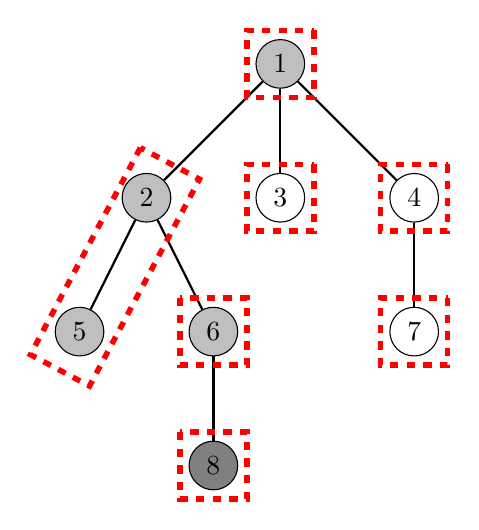
\begin{tikzpicture}[scale=0.85]
\node[draw, circle, fill=lightgray] (1) at (0,3) {$1$};
\node[draw, circle] (2) at (2,1) {$4$};
\node[draw, circle, fill=lightgray] (3) at (-2,1) {$2$};
\node[draw, circle] (4) at (0,1) {$3$};
\node[draw, circle] (5) at (2,-1) {$7$};
\node[draw, circle, fill=lightgray] (6) at (-3,-1) {$5$};
\node[draw, circle, fill=lightgray] (7) at (-1,-1) {$6$};
\node[draw, circle, fill=gray] (8) at (-1,-3) {$8$};
\path[draw,thick,-] (1) -- (2);
\path[draw,thick,-] (1) -- (3);
\path[draw,thick,-] (1) -- (4);
\path[draw,thick,-] (2) -- (5);
\path[draw,thick,-] (3) -- (6);
\path[draw,thick,-] (3) -- (7);
\path[draw,thick,-] (7) -- (8);

\draw [red,thick,dashed,line width=2pt,rotate around={-28:(-2,0)}] (-2.9,1.5) rectangle (-1.9,-2);


\draw [red,thick,dashed,line width=2pt] (-1.5,-0.5) rectangle (-0.5,-1.5);
\draw [red,thick,dashed,line width=2pt] (-1.5,-2.5) rectangle (-0.5,-3.5);

\draw [red,thick,dashed,line width=2pt] (0.5,3.5) rectangle (-0.5,2.5);
\draw [red,thick,dashed,line width=2pt] (0.5,1.5) rectangle (-0.5,0.5);
\draw [red,thick,dashed,line width=2pt] (2.5,1.5) rectangle (1.5,0.5);
\draw [red,thick,dashed,line width=2pt] (2.5,-0.5) rectangle (1.5,-1.5);
\end{tikzpicture}
\end{center}

Kasnije, pri posjetu čvora 7,
algoritam utvrđuje da je
najniži zajednički predak čvorova 2 i 7 jednak 1:
\begin{center}
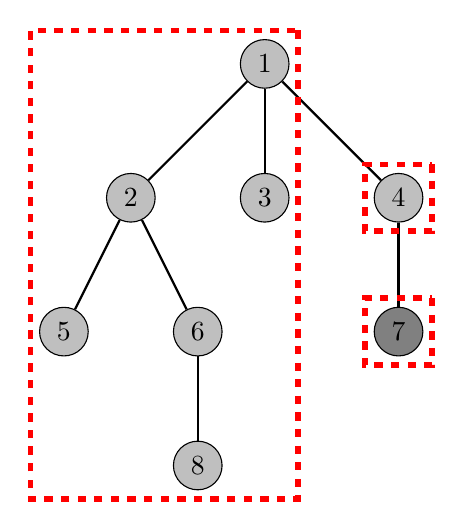
\begin{tikzpicture}[scale=0.85]
\node[draw, circle, fill=lightgray] (1) at (0,3) {$1$};
\node[draw, circle, fill=lightgray] (2) at (2,1) {$4$};
\node[draw, circle, fill=lightgray] (3) at (-2,1) {$2$};
\node[draw, circle, fill=lightgray] (4) at (0,1) {$3$};
\node[draw, circle, fill=gray] (5) at (2,-1) {$7$};
\node[draw, circle, fill=lightgray] (6) at (-3,-1) {$5$};
\node[draw, circle, fill=lightgray] (7) at (-1,-1) {$6$};
\node[draw, circle, fill=lightgray] (8) at (-1,-3) {$8$};
\path[draw,thick,-] (1) -- (2);
\path[draw,thick,-] (1) -- (3);
\path[draw,thick,-] (1) -- (4);
\path[draw,thick,-] (2) -- (5);
\path[draw,thick,-] (3) -- (6);
\path[draw,thick,-] (3) -- (7);
\path[draw,thick,-] (7) -- (8);

\draw [red,thick,dashed,line width=2pt] (0.5,3.5) rectangle (-3.5,-3.5);
\draw [red,thick,dashed,line width=2pt] (2.5,1.5) rectangle (1.5,0.5);
\draw [red,thick,dashed,line width=2pt] (2.5,-0.5) rectangle (1.5,-1.5);

\end{tikzpicture}
\end{center}
